\chapter{Fundamental}
\label{ch:fundamental}

%%%%%%%%%%%%%%%%%%%%%%%%%%%%%%%%%%%%%%%%%%%%%%%%%%%%%%%%%%%%%%%%%%%%%%%%%%%%%%%%%%%%%%%%%%%%%%%%%%%%%%%%%%%%%%%%%%%%%%%%%%%%%%
Inverted pendulums, as indicated at the issue's outset, 
are common scientific items and find usage in various practical contexts.
Model system construction by ifas is described in detail in Sections \ref{sec:Mecsys}
and \ref{sec:Hydsys} of this chapter. Then, the fundamentals of mechanics and 
hydrodynamics for a realistic model are implemented in Section 1.3. 
The controller design is explored in detail in Section 1.4.

%%%%%%%%%%%%%%%%%%%%%%%%%%%%%%%%%%%%%%%%%%%%%%%%%%%%%%%%%%%%%%%%%%%%%%%%%%%%%%%%%%%%%%%%%%%%%%%%%%%%%%%%%%%%%%%%%%%%%%%%%%%%%%

\section{Mechanical system} %without '*' will get a subsection with number "3.1, 3.2"
\label{sec:Mecsys}

The pendulum consists of a cylinder and a pole, 
one end of the pole is inserted into the cylinder,
and the other end is connected to the cart via a revolute joint,
this joint allows the pendulum to rotate at least 360° during 
the movement of the cart. A rail which runs across the cart ensures that 
the cart's motion is restricted sideways sliding only. As seeing from Fig \ref*{fig:pendulum}.\\
\begin{figure}[htbp]
    \centering
    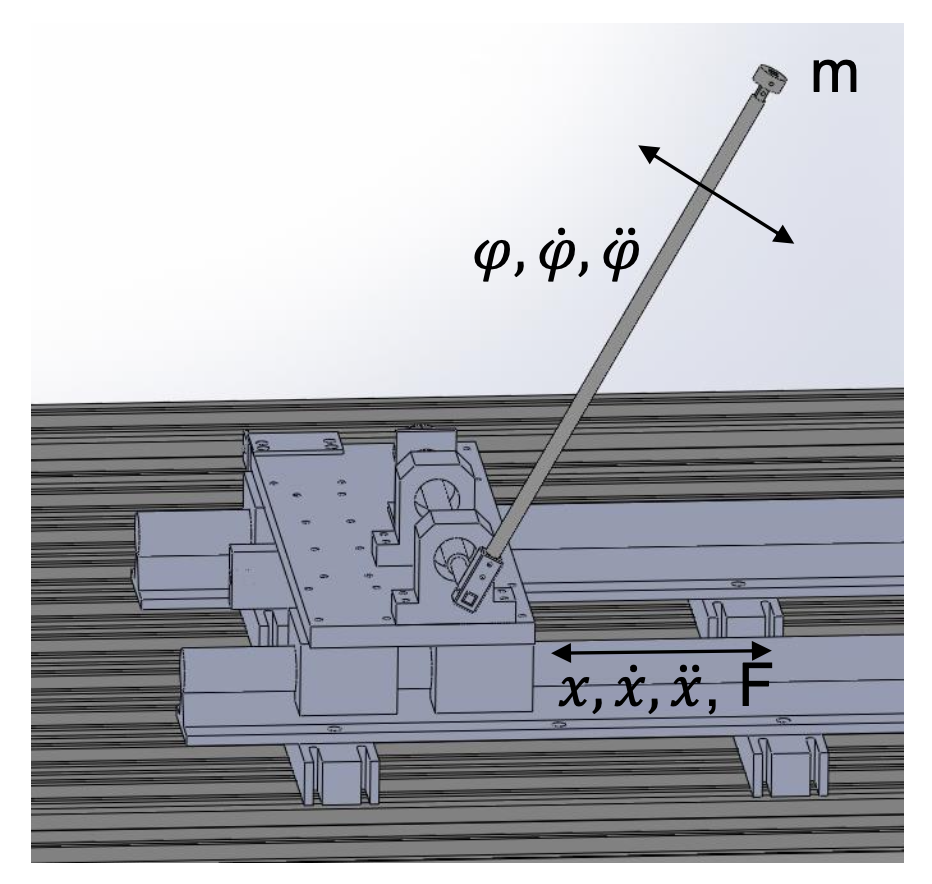
\includegraphics[width = 0.3\textwidth]{pendulum.png}
    \caption[Inverse pendulum sketch]{sketch of inverse pendulum (\cite[]{skependel})
    \label{fig:pendulum}} %label should over the caption and then to ref.
\end{figure}\\
A sensor mounted on the joint measures the angle of the pendulum, and the sensor data is sent 
to the controller for claculate until the angle \ensuremath{\phi} reaches vertical equilibrium, aka. 0°.

%%%%%%%%%%%%%%%%%%%%%%%%%%%%%%%%%%%%%%%%%%%%%%%%%%%%%%%%%%%%%%%%%%%%%%%%%%%%%%%%%%%%%%%%%%%%%%%%%%%%%%%%%%%%%%%%%%%%%%%%%%%%%%
\section{Hydraulic system}
\label{sec:Hydsys}
The hydraulic system is built by ifas. This system consists of a pump, a tank, 
a hydraulic cylinder, a capsule accumulator, and a 4/3 servo valve as its primary components. \\
A hydraulic cylinder, also known as a linear hydraulic motor, is powered by the                                                                                             
incompressible liquid hydraulic fluid compressed within the cylinder. 
By altering the pressure on both sides of the piston, the piston is pushed to move from 
side to side, therefore propelling the piston rod. Sketc.h will be showen form Fig \ref*{fig:hydcylinder}.\\
\begin{figure}[htbp]
  \centering
  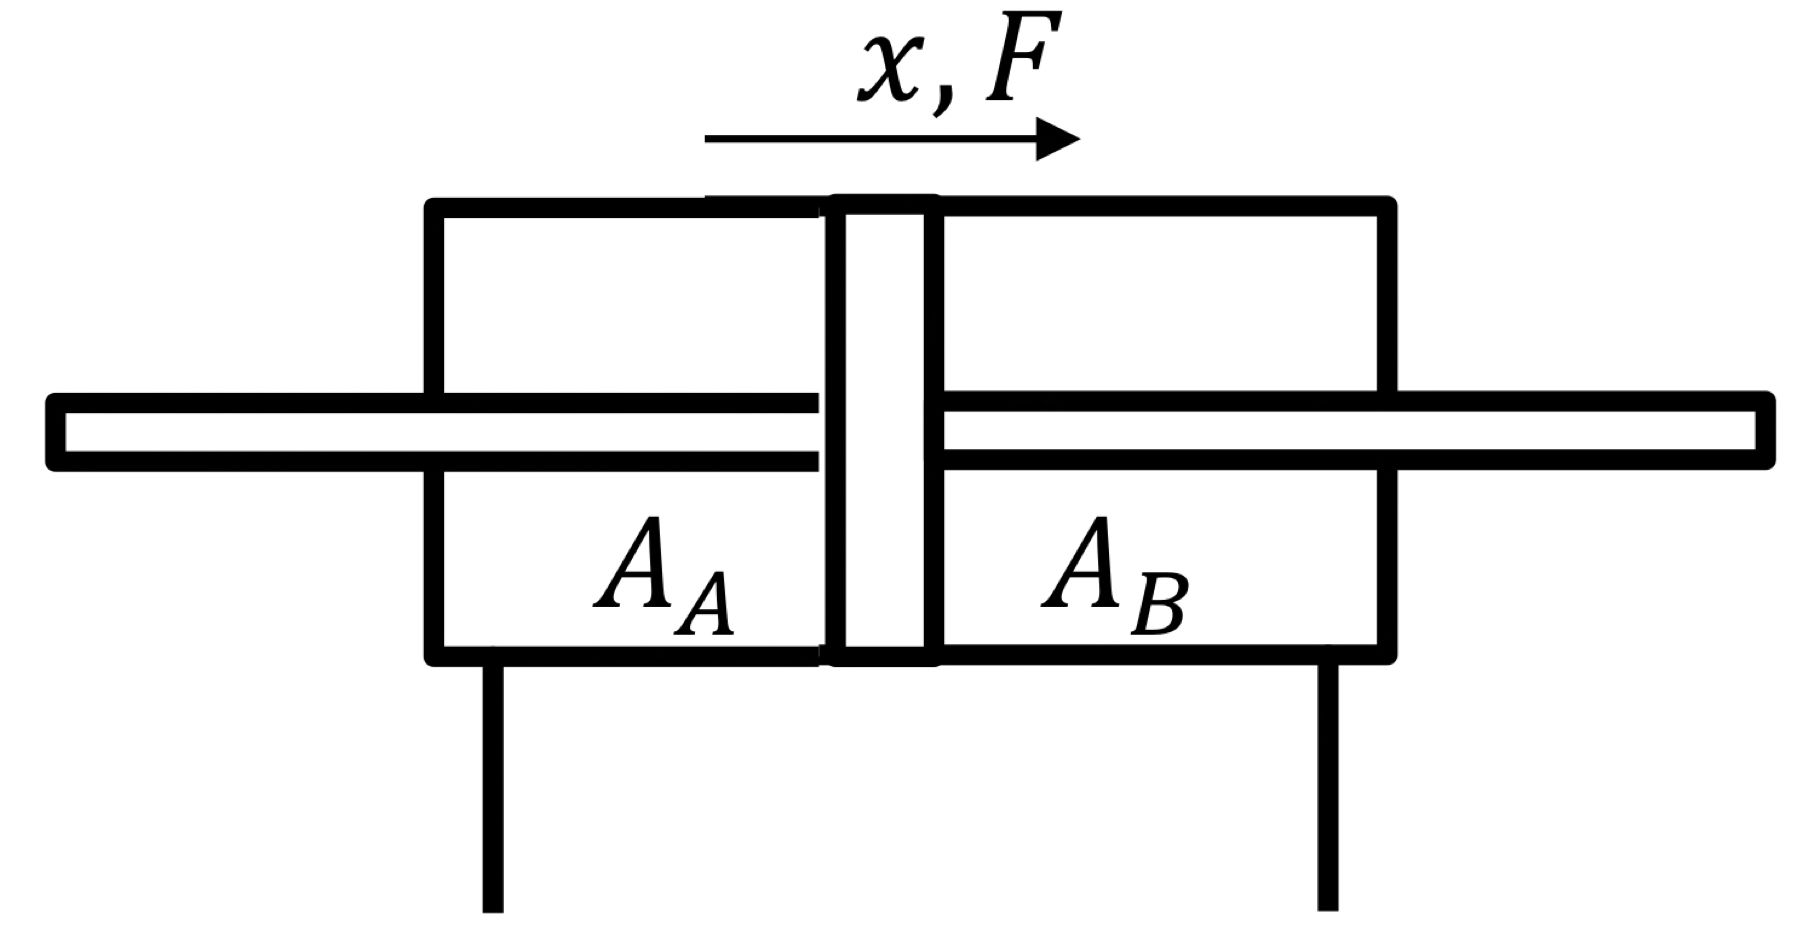
\includegraphics[width = 0.2\textwidth]{Contents/Resources/hydcylinder.jpeg}
  \caption[Hydraulic cylinder sketch]{Sketch of hydraulic cylinder}
  \label{fig:hydcylinder}
\end{figure}\\
Why would a hydraulic system be used to drive a cart instead of an electric motor? 
Hydraulics provides a simple yet effective method for generating a great deal of force 
in a small area, which was designed fairly early on and requires 
just a very tiny apparatus to raise 1 or 2 tons of objects with using the hydraulic force. 
Due to the incompressibility of hydraulic oil, the oil in the cylinder resembles a 
solid at high pressure, which gives the Hydraulic cylinder excellent dynamic properties.\\
\begin{figure}[htbp]
  \centering
  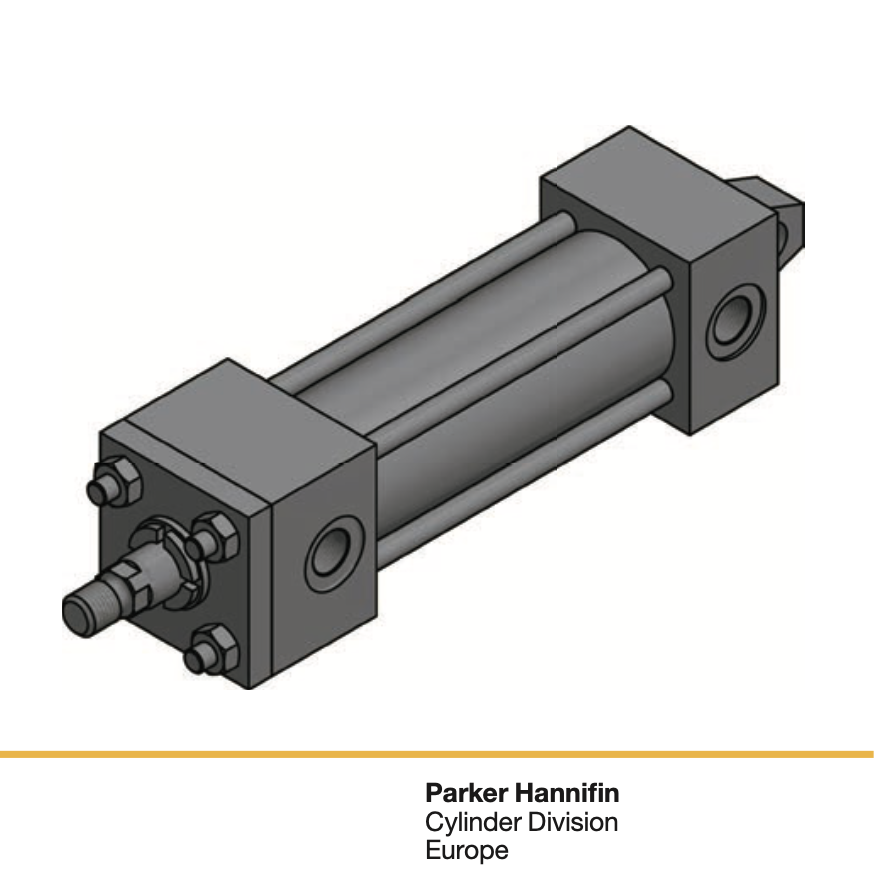
\includegraphics[width = 0.4\textwidth]{Contents/Resources/Parker Hydcylinder.png}
  \caption[Parker® Hydraulic cylinder]{Parker® hydraulic cylinder HMI-ME6(\cite[]{parker})}
  \label{fig:Parker}
\end{figure}\\
Existing hydraulic cylinder can provide working pressure up to 700bar. The hydraulic
cylinder in the unit is supplied by Parker® and the model HMI-ME6 can work up to 210 bar.
